%%%%%%%%%%%%%%%%%%%%%%%%%%%%%%%%%%%%%%%%%%%%%%%%%%%%%%%%%%%%%%%%%%%%%%%
% Author: Miguel Ferreira e Vanessa Silva                             %
% Info:                                                               %
% Language: Portuguese                                                %
%%%%%%%%%%%%%%%%%%%%%%%%%%%%%%%%%%%%%%%%%%%%%%%%%%%%%%%%%%%%%%%%%%%%%%%

\documentclass[a4paper,11pt,pdftex]{article}
\usepackage[T1]{fontenc}
\usepackage[portuguese]{babel}
\usepackage[utf8]{inputenc}
\usepackage{fullpage}
\usepackage[top=2.5cm, bottom=2.5cm, left=2.5cm , right=2.5cm]{geometry}
\usepackage{marginnote}        %use \marginnote{}
\usepackage[pdftex]{graphicx}  %Support for images in pdf
\usepackage{hyperref} 	       %Support for hyperlinks in pdf
\usepackage{textcomp}
\usepackage{tikz}
%\usepackage{times}            %times font
\usepackage{pdfpages} % Include a pdf page
\usepackage{caption}
\usepackage{subcaption}
\usepackage{verbatim}
\usepackage{color}
\usepackage{listings}          %for simple inclusion of source code
\usepackage[cc]{titlepic}      %glider on title page
\usepackage{url}
%\usepackage{natbib}
\usepackage{rotating}
\usepackage{lipsum}
\usepackage{fancyhdr}
\usepackage[portuguese,ruled]{algorithm2e}
\usepackage[noend]{algpseudocode}
\usepackage{footnote}
\usepackage{amsfonts}
\usepackage{mathtools}
\definecolor{dkgreen}{rgb}{0,0.6,0}
\definecolor{gray}{rgb}{0.5,0.5,0.5}
\definecolor{mauve}{rgb}{0.58,0,0.82}
\definecolor{lightgrey}{RGB}{238,238,238}

\usepackage{enumerate}

%%%%%%%%%%%%%%%%%%%%IMPORTANTE COMMANDS I FORGET%%%%%%%%%%%%%%%%%%%%%%%
% \marginnote                                                         %
% \footnote                                                           %
% \hiperlink{tag}{text} & hypertarget{tag}{text}                      %
%%%%%%%%%%%%%%%%%%%%%%%%%%%%%%%%%%%%%%%%%%%%%%%%%%%%%%%%%%%%%%%%%%%%%%%
% [hidelinks] doesn't work so:                                        %
%                                                                     %
%  \hypersetup{                                                       %
%   colorlinks=false,                                                 %
%  pdfborder={0 0 0},                                                 %
%  }                                                                  %
% \framebox[\linewidth][l]{                                           %
% \lstinputlisting[title=HelloWorld.c]{./Programs/HelloWorld.c}       %
% }                                                                   %
%\includepdf[pages={{},{1},{},{2},{},{3},{},{4},{},{5},{},{6},{},{7}, %
%{},{8},{},{9},{},{10},{},{11},{},{12}},pagecommand={\thispagestyle{  %
% fancy}}]{script}                                                    %
%%%%%%%%%%%%%%%%%%%%%%%%%%%%%%%%%%%%%%%%%%%%%%%%%%%%%%%%%%%%%%%%%%%%%%%

\title{Trabalho 5 - VLAN e SNMP}

\author{Miguel Ferreira\\
  \href{mailto:miguelferreira108@gmail.com}{\texttt{miguelferreira108@gmail.com}}\\
  Vanessa Silva\\
  \href{mailto:up201305731@fc.up.pt}{\texttt{up201305731@fc.up.pt}}\\
\multicolumn{1}{p{.7\textwidth}}{\centering\emph{
\\Administração de Redes,\\Departamento de Ciências de Computadores,\\Faculdade de Ciências da Universidade do Porto}}
}
\date{\today}
%\titlepic{
%}

%%%%%%%%%%%%%%%%%%%%%%%%%%%%% SETTINGS %%%%%%%%%%%%%%%%%%%%%%%%%%%%%%%%
\lstset{
  language=C,   % choose the language of the code
  numbers=left,        % where to put the line-numbers
  stepnumber=1,        % the step between two line-numbers.        
  numbersep=8pt,       % how far the line-numbers are from the code
  backgroundcolor=\color{lightgrey}, % \usepackage{color}
  showspaces=false,    % show spaces adding particular underscores
  showstringspaces=false,        % underline spaces within strings
  showtabs=false,      % show tabs within strings adding underscores
  tabsize=2,           % sets default tabsize to 2 spaces
  captionpos=b,        % sets the caption-position to bottom
  breaklines=true,     % sets automatic line breaking
  breakatwhitespace=true, % if automatic breaks only happen atwhitespace
  title=\lstname,      % show the filename of files \lstinputlisting;
  frame=single,
  keywordstyle=\color{blue},          % keyword style
  commentstyle=\color{dkgreen},       % comment style
  stringstyle=\color{mauve},
  basicstyle=\ttfamily,
}
\hypersetup{
    bookmarks=true,         % show bookmarks bar?
    unicode=true,          % non-Latin characters in Acrobat’sbookmarks
    pdftoolbar=true,        % show Acrobat’s toolbar?
    pdfmenubar=true,        % show Acrobat’s menu?
    pdffitwindow=false,     % window fit to page when opened
    pdfstartview={FitH},    % fits the width of the page to the window
    pdftitle={Título},    % title
    pdfauthor={Miguel Ferreira e Vanessa Silva},                        % author
    pdfcreator={Miguel Ferreira e Vanessa Silva},   % creator of the document
%     pdfproducer={Producer}, % producer of the document
%     pdfkeywords={keyword1} {key2} {key3}, % list of keywords
%     pdfnewwindow=true,      % links in new window
%     colorlinks=false,       % false: boxed links; true: colored links
%     linkcolor=red,          % color of internal links
%     citecolor=green,        % color of links to bibliography
%     filecolor=magenta,      % color of file links
%     urlcolor=cyan           % color of external links
}

%%%%%%%%%%%%%%%%%%%%%%%%%% END SETTINGS %%%%%%%%%%%%%%%%%%%%%%%%%%%%%%%
\begin{document}
\maketitle
%\tableofcontents
\section*{Introdução}

No âmbito da unidade curricular de Administração de Redes, implementamos a rede da figura abaixo, em que R1 é um router Cisco 2691 com um módulo de comutação de 16 portas.\\

\begin{figure}[h]
\centering
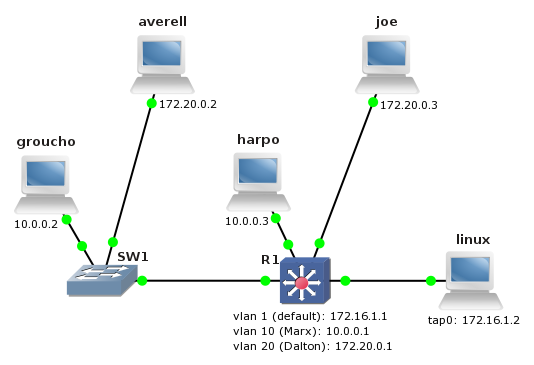
\includegraphics[width=0.7\textwidth, height=0.3\textheight]{rede.png}
\label{fig:rede}
\caption{Rede implementada na aula.}
\end{figure}

\newpage
\section*{Questões}
\paragraph{1.}

\subparagraph{a.}
Captura do primeiro ICMP \emph{Echo Request} enviado em ambas as interfaces:

\begin{figure}[h]
\centering
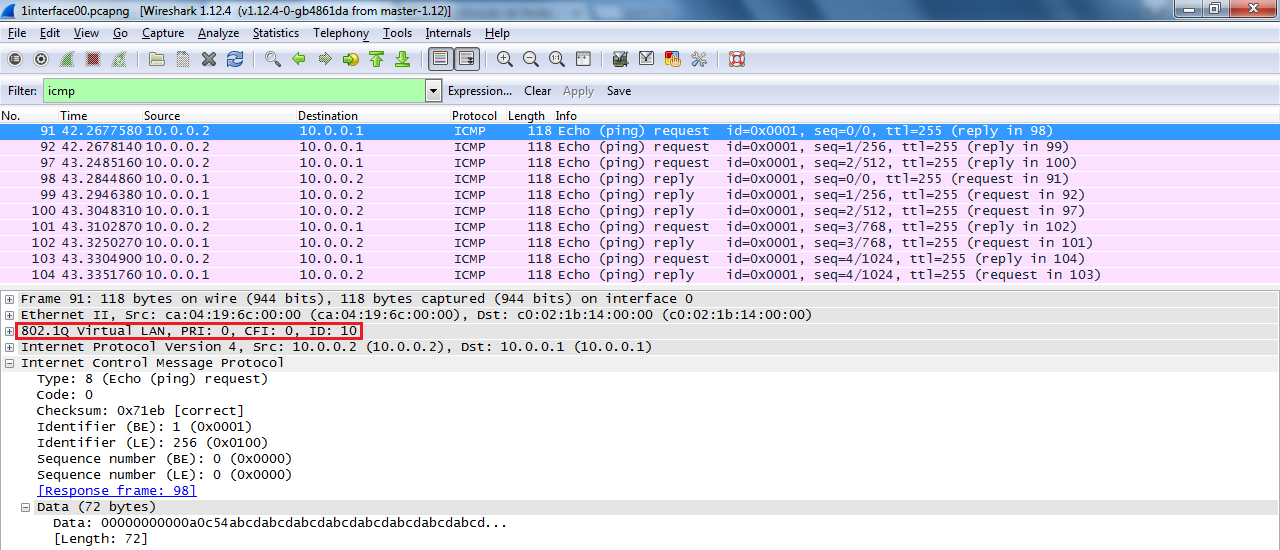
\includegraphics[width=1\textwidth, height=0.32\textheight]{1_interface00-groucho.png}
\label{fig:2-capturaWireshark}
\caption{Captura \emph{wireshark} na interface \textsf{f0/0} de \textsf{groucho}.}
\end{figure}

\begin{figure}[h]
\centering
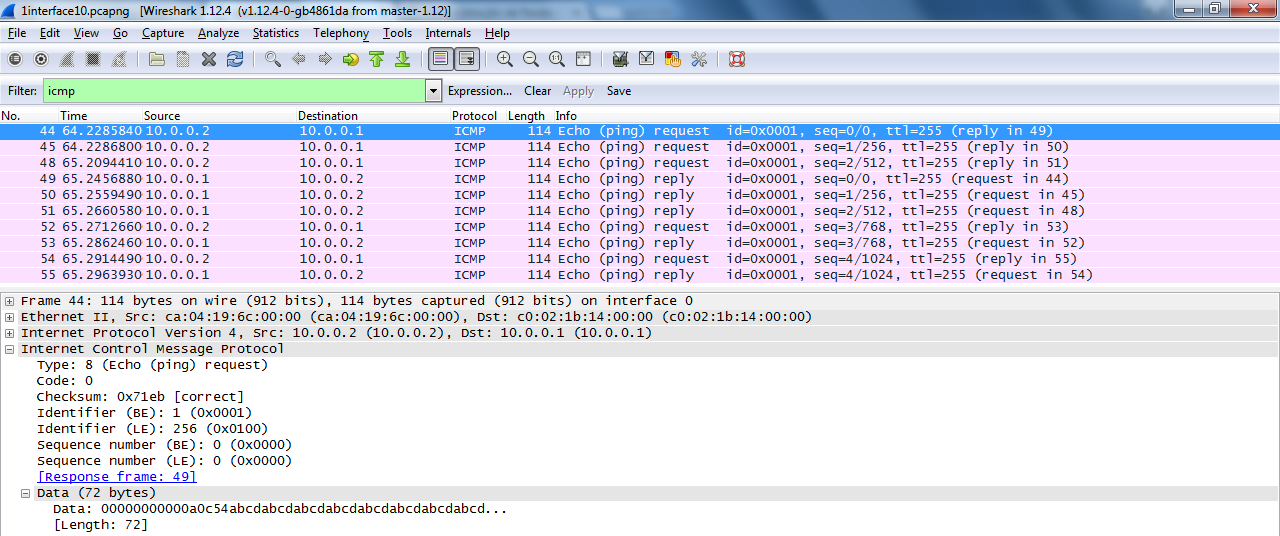
\includegraphics[width=1\textwidth, height=0.32\textheight]{1_interface10-R1.png}
\label{fig:3-capturaWireshark}
\caption{Captura \emph{wireshark} na interface \textsf{f1/0} de \textsf{R1}.}
\end{figure}


\subparagraph{b.}
Quais foram as diferenças encontradas e a que se devem? (texRes)

%no primeiro ICMP \emph{Echo Request} enviado na interface de R1 encontra-se um encapsulamento diferente 802.1Q (portas trunk), ao contrário de na intergace do groucho.


\paragraph{2.}
Na interface \textsf{f1/0} de \textsf{R1} podemos observar que é enviadas várias
mensagens ARP (ARP \emph{Request}) em \emph{Broadcast}, 
(\texttt{Who has 10.0.0.2? Tell 10.0.0.4}), que significa que o \emph{host} 
10.0.0.4 está a tentar descobrir quem é a máquina 10.0.0.2, à qual não se obteve
nenhuma resposta.

Isto acontece porque as portas de \textsf{SW1} estão configuradas em 
\textbf{modo acesso} na VLAN 10 (\textsf{groucho}) e na VLAN20  (\textsf{averell}), 
apesar de ambos os IPs (de \textsf{groucho} e \textsf{averell}) pertencerem à mesma subnet, o \texttt{ping} nunca chega à máquina do \textsf{groucho} (na captura 
\emph{wireshark} na interface \textsf{f0/0} não chega nenhuma mensagem) uma vez que 
as máquinas pertencem a VLANs diferentes.


\paragraph{3.}
 Faça um ping de groucho para averell. O que observa em relação aos pacotes ICMP? (capRes + texRes)
 
\begin{figure}[h]
\centering
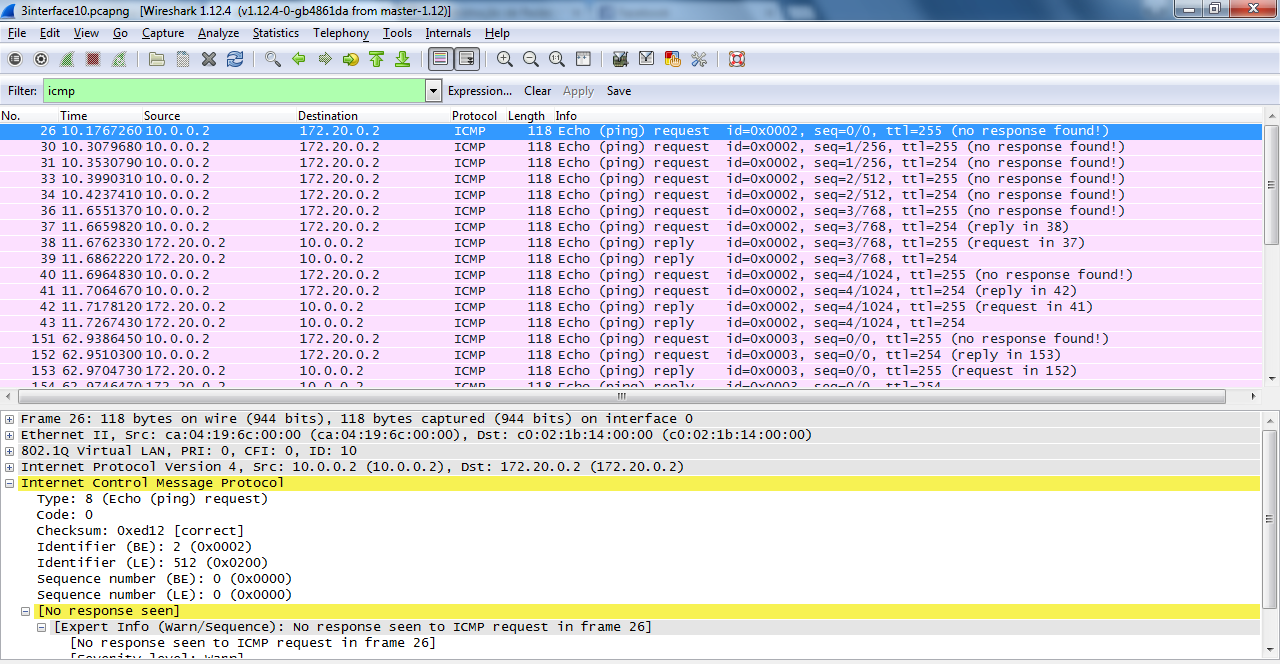
\includegraphics[width=1\textwidth, height=0.38\textheight]{3_interface10_R1.png}
\label{fig:4-capturaWireshark}
\caption{Captura \emph{wireshark} na interface \textsf{f1/0} de \textsf{R1}.}
\end{figure}


\paragraph{4.}

\subparagraph{a.}
Para que a ligação entre \textsf{R1} e o terminal \textsf{linux} funcione em modo \emph{trunk} tivemos de realizar as seguintes configurações.

No \emph{router} \textsf{R1}:
\begin{verbatim}
interface FastEthernet 1/3
switchport trunk encapsulation dot1q
switchport mode trunk
\end{verbatim}

No terminal \textsf{linux}:
\begin{verbatim}
[root@Labs5610 ar]# modprobe 8021q
[root@Labs5610 ar]# vconfig add tap0 10
Added VLAN with VID == 10 to IF -:tap0:-
[root@Labs5610 ar]# 
[root@Labs5610 ar]# ifconfig tap0.10 10.0.0.5 netmask 255.255.255.0 up
\end{verbatim}


\subparagraph{b.}
Captura de um pacote do \textsf{ping} (ICMP) enviado em ambas as interfaces:

\begin{figure}[h]
\centering
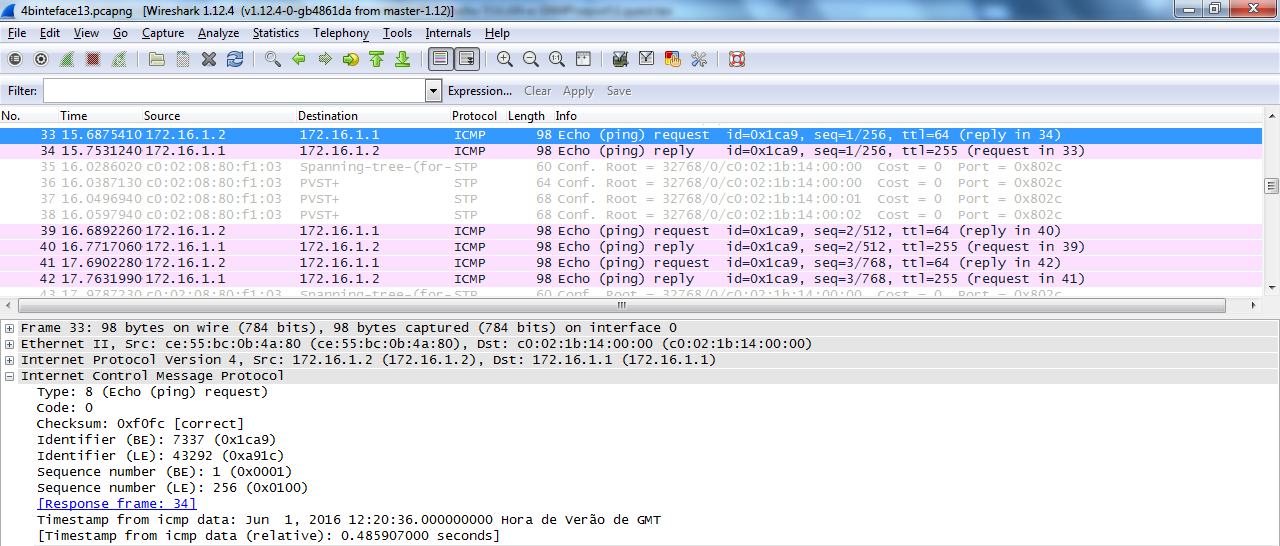
\includegraphics[width=1\textwidth, height=0.33\textheight]{4_ping_VLAN1.png}
\label{fig:5-capturaWireshark}
\caption{Captura \emph{wireshark} de um pacote do \texttt{ping} enviado do terminal \textsf{linux} para a \textsf{VLAN 1}.}
\end{figure}

\begin{figure}[h]
\centering
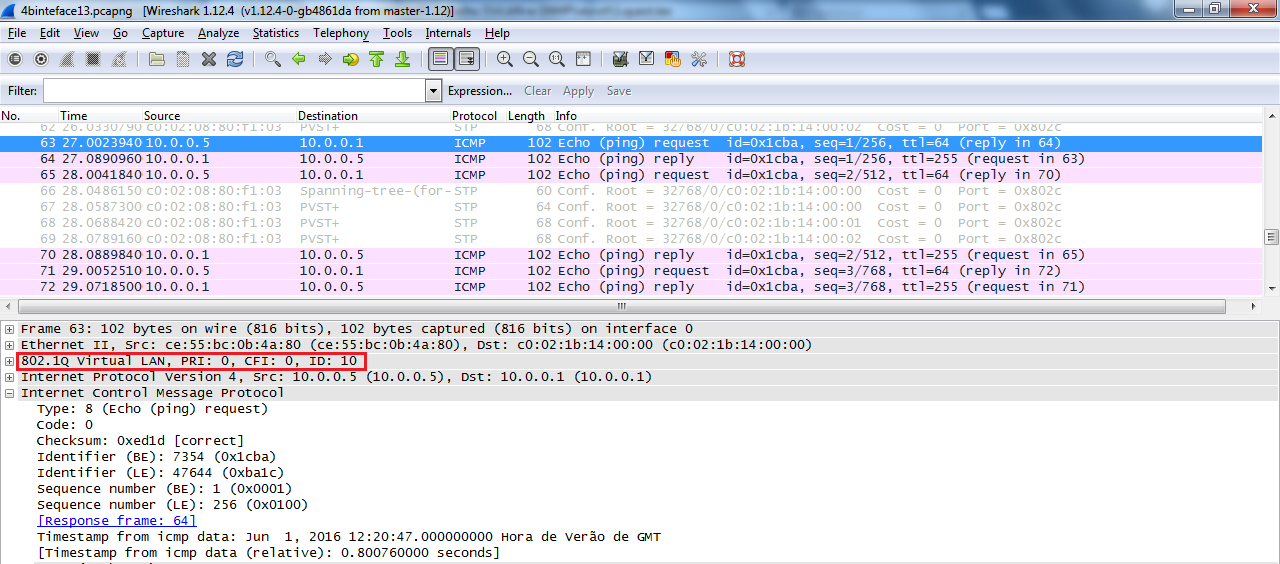
\includegraphics[width=1\textwidth, height=0.33\textheight]{4_ping_VLAN10.png}
\label{fig:6-capturaWireshark}
\caption{Captura \emph{wireshark} de um pacote do \texttt{ping} enviado do terminal \textsf{linux} para a \textsf{VLAN 10}.}
\end{figure}


\subparagraph{c.}
Como explica o que observou na alínea anterior? (texRes)


\paragraph{5.}

\subparagraph{a.}
\begin{verbatim}
[root@Labs5610 ar]# snmpget -v 2c -c Leitura 172.16.1.1 iso.org.dod.internet.mgmt.mib-2.system.sysDescr
SNMPv2-MIB::sysDescr = No Such Instance currently exists at this OID
\end{verbatim}

Não se conseguiu realizar o \texttt{get} porque foi solicitada uma classe e não uma instância.

Quando queremos usar um OID precisamos de adicionar um outro número para obter o valor dessa variável. Por isso, precisamos de acrescentar um \texttt{.0} que representa a primeira instância desse objeto.


\subparagraph{b.}
\begin{verbatim}
[root@Labs5610 ar]# snmpget -v 2c -c Leitura 172.16.1.1 iso.org.dod.internet.mgmt.mib-2.system.sysDescr.0
SNMPv2-MIB::sysDescr.0 = STRING: Cisco IOS Software, 2600 Software (C2691-ADVIPSERVICESK9-M), Version 12.4(15)T6, RELEASE SOFTWARE (fc2)
Technical Support: http://www.cisco.com/techsupport
Copyright (c) 1986-2008 by Cisco Systems, Inc.
Compiled Mon 07-Jul-08 04:30 by prod_rel_team
\end{verbatim}


\subparagraph{c.}
O \texttt{getnext} serve para retornar a instância da classe OID, na árvore de MIB de dados, a seguir à instância descrita no comando. Ou seja, retorna o valor da variável sucessora lexicográfica.


\begin{verbatim}
[root@Labs5610 ar]# snmpgetnext -v 2c -c Leitura 172.16.1.1 iso.org.dod.internet.mgmt.mib-2.system.sysDescr.0
SNMPv2-MIB::sysObjectID.0 = OID: SNMPv2-SMI::enterprises.9.1.122
\end{verbatim}


\subparagraph{d.}
O \texttt{walk} percorre todas as instâncias de todas as classes respeitando a hierarquia. É construído de  acordo com  as  respostas  que  vai  recebendo  do  \texttt{get-next-request} (ver  na captura abaixo) para recolher a informação a seguir.

Ou seja, o objetivo é recupera uma sub-árvore de valores usando repetidas solicitações SNMP GetNext. 
Se é dado um OID, este especifica qual parte do espaço serão pesquisadas usando as solicitações \texttt{getnext}. Todas as variáveis ​​na sub-árvore abaixo desse OID serão consultadas e os seus valores apresentados para o usuário.
Se não é dados nenhum OID, o \texttt{walk} irá procurar a sub-árvore a partir de SNMPv2-SMI :: mib-2.
O \texttt{walk} para quando retorna resultados que já não estão dentro do alcance do OID.

\begin{figure}[h]
\centering
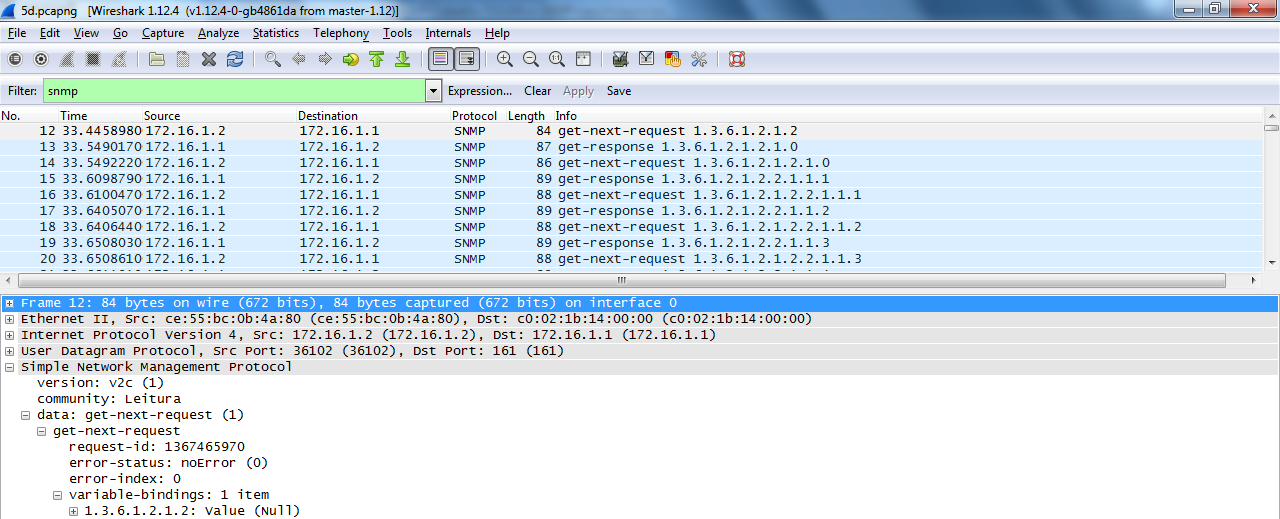
\includegraphics[width=1\textwidth, height=0.33\textheight]{5d.png}
\label{fig:7-capturaWireshark}
\caption{Captura \emph{wireshark} de pacotes SNMP na interface \textsf{f1/3} de \textsf{R1}.}
\end{figure}


\subparagraph{e.}
Com base nos resultados da alínea anterior, diga quantas interfaces tem o router e quais são elas. (texRes)

O \emph{router} tem 22 interfaces, que são as que se seguem (parte da resposta do \texttt{snmpwalk} no terminal \textsc{linux}):

\begin{verbatim}
IF-MIB::ifNumber.0 = INTEGER: 22
...
IF-MIB::ifDescr.1 = STRING: FastEthernet0/0
IF-MIB::ifDescr.2 = STRING: FastEthernet0/1
IF-MIB::ifDescr.3 = STRING: FastEthernet1/0
IF-MIB::ifDescr.4 = STRING: FastEthernet1/1
IF-MIB::ifDescr.5 = STRING: FastEthernet1/2
IF-MIB::ifDescr.6 = STRING: FastEthernet1/3
IF-MIB::ifDescr.7 = STRING: FastEthernet1/4
IF-MIB::ifDescr.8 = STRING: FastEthernet1/5
IF-MIB::ifDescr.9 = STRING: FastEthernet1/6
IF-MIB::ifDescr.10 = STRING: FastEthernet1/7
IF-MIB::ifDescr.11 = STRING: FastEthernet1/8
IF-MIB::ifDescr.12 = STRING: FastEthernet1/9
IF-MIB::ifDescr.13 = STRING: FastEthernet1/10
IF-MIB::ifDescr.14 = STRING: FastEthernet1/11
IF-MIB::ifDescr.15 = STRING: FastEthernet1/12
IF-MIB::ifDescr.16 = STRING: FastEthernet1/13
IF-MIB::ifDescr.17 = STRING: FastEthernet1/14
IF-MIB::ifDescr.18 = STRING: FastEthernet1/15
IF-MIB::ifDescr.20 = STRING: Null0
IF-MIB::ifDescr.21 = STRING: Vlan1
IF-MIB::ifDescr.22 = STRING: Vlan10
IF-MIB::ifDescr.23 = STRING: Vlan20
...
\end{verbatim}


\subparagraph{f.}
Resultado do \texttt{get}:
\begin{verbatim}
[root@Labs5610 ar]# snmpget -v 2c -c Leitura 172.16.1.1 iso.org.dod.internet.mgmt.mib-2.system.sysName.0
SNMPv2-MIB::sysName.0 = STRING: R1
\end{verbatim}

Comando usado para fazer o \texttt{set}:
\begin{verbatim}
[root@Labs5610 ar]# snmpset -v 2c -c Escrita 172.16.1.1 iso.org.dod.internet.mgmt.mib-2.system.sysName.0 s R2
SNMPv2-MIB::sysName.0 = STRING: R2
\end{verbatim}


\subparagraph{g.}
Faça um walk e um bulkwalk à sub-árvore system da MIB-2. Qual é a diferença entre estes dois comandos e em que se traduz na prática? (2×capRes + texRes)

O \texttt{bulkwalk} obtém a informação com apenas um pedido, uma vez que usa solicitações SNMP GetBulk (\texttt{get-bulk-request} permite a transferência de grandes volumes de informação). Enquanto que o \texttt{walk} usa solicitações SNMP GetNext, que realiza um pedido para cada variável. A vantagem é o ganho em termos de eficiência.Podemos  ver  a  diferença  na  quantidade  de  pedidos  entre  os  2,  através  das  setas  a vermelho nas capturas

get-next-pedido retorna o item na MIB logo após o item especificado . 

snmpbulkwalk é uma aplicação SNMP que usa solicitações SNMP GetBulk para consultar uma entidade de rede de forma eficiente.


A operação GetBulk é normalmente usada para recuperar grande quantidade de dados. Um pedido GetBulk é feito dando uma lista OID junto com um valor Max-repetições e um valor Nonrepeaters.
 
A operação GetBulk executa uma operação contínua GETNEXT com base no valor Max-repetições. O valor Nonrepeaters determina o número de variáveis ​​na lista de variáveis ​​para as quais uma operação GETNEXT simples tem de ser feito. Para as demais variáveis, a operação GETNEXT contínua é feito com base no valor Max-Repetições.
 
Em outras palavras, a operação SNMP GetBulk faz uma operação GETNEXT simples para as primeiras ligações variável n no pedido e faz operação de M GETNEXT (contínua) para cada um dos restantes ligações de R variáveis ​​na lista de pedidos onde

N é o mínimo de
o valor do campo não repetidores no pedido
o número de ligações de variáveis ​​no pedido
M é o campo Max-repetições do pedido
 
R é o máximo de
o número de ligações de variáveis ​​no pedido
zero
Assim, o número total de varbinds na mensagem de resposta é (N + H x R).



\begin{figure}[h]
\centering
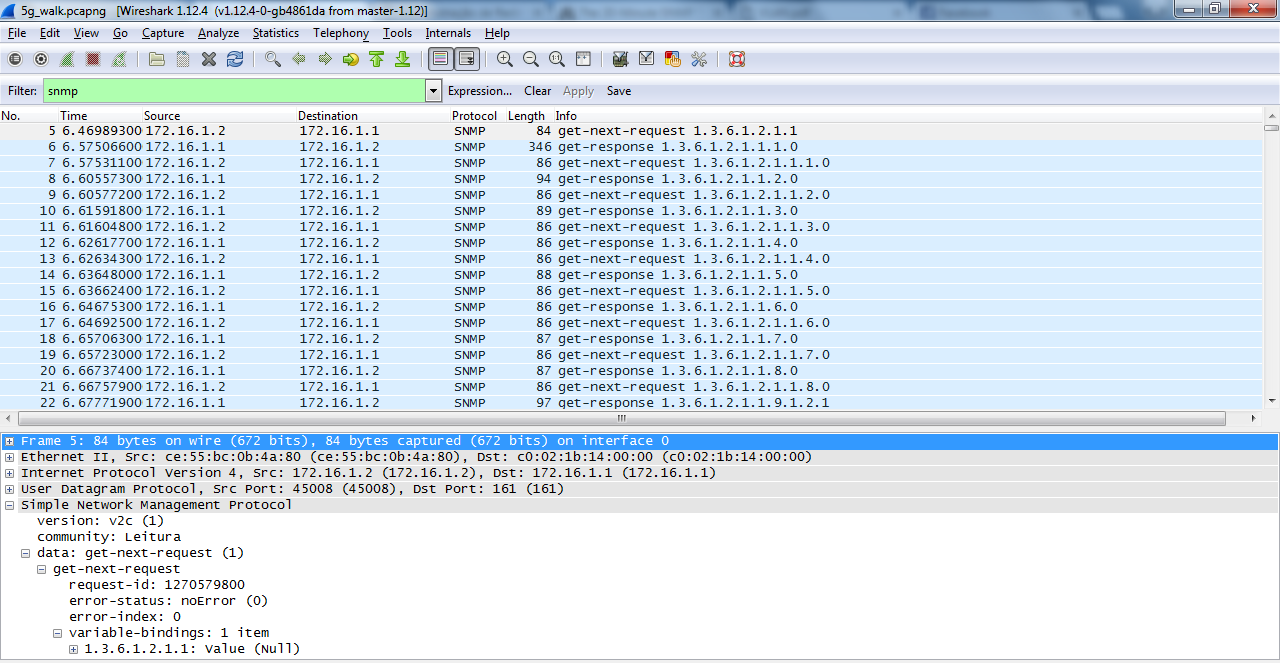
\includegraphics[width=1\textwidth, height=0.33\textheight]{5g_walk.png}
\label{fig:8-capturaWireshark}
\caption{Captura \emph{wireshark} de pacotes \texttt{snmpwalk}.}
\end{figure}

\begin{figure}[h]
\centering
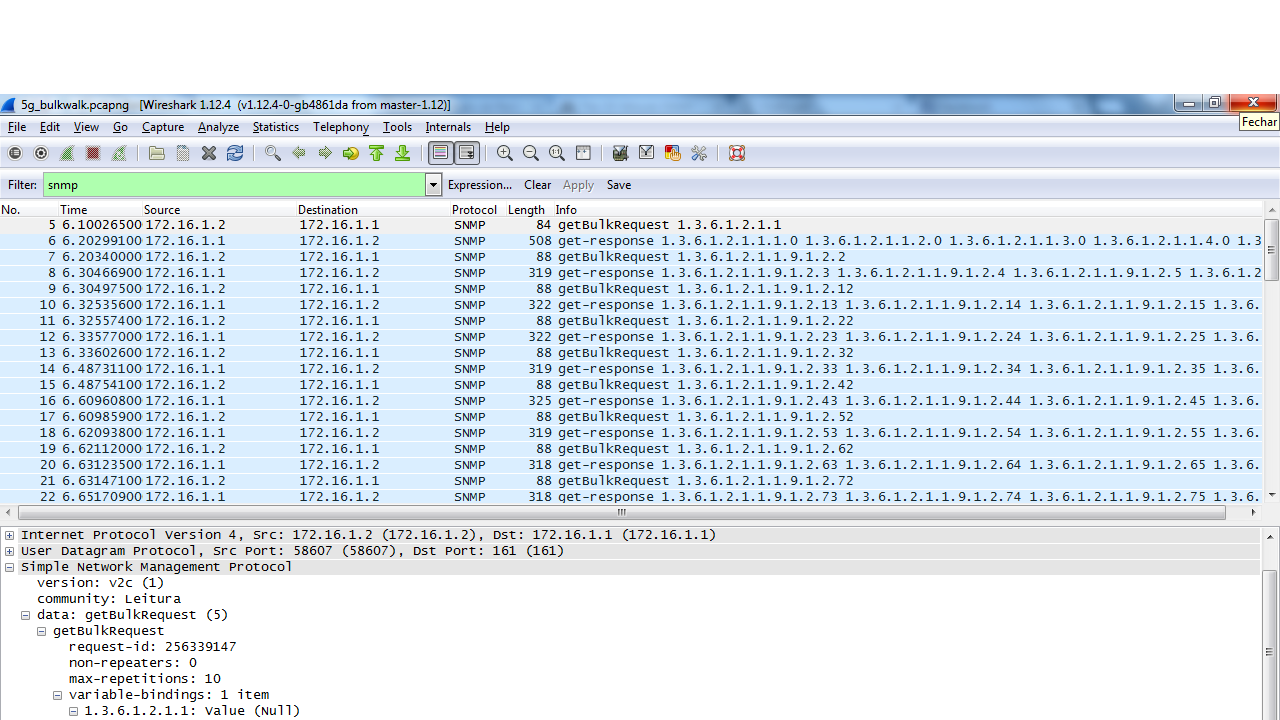
\includegraphics[width=1\textwidth, height=0.33\textheight]{5g_bulkwalk.png}
\label{fig:9-capturaWireshark}
\caption{Captura \emph{wireshark} de pacotes \texttt{bulkwalk}.}
\end{figure}


\subparagraph{h.}
Informação sobre as interfaces de \textsf{R1}:
\begin{verbatim}
[root@Labs5610 ar]# snmpnetstat -v 2c -Ci -c Leitura 172.16.1.1
Name      Mtu Network     Address    Ipkts Ierrs Opkts Oerrs Queue
Fa0/0    1500                            0     0     0     0     0
Fa0/1    1500                            0     0     0     0     0
Fa1/0    1500                            0     0     0     0     0
Fa1/1    1500                            0     0     0     0     0
Fa1/2    1500                            0     0     0     0     0
Fa1/3    1500                            0     0     0     0     0
Fa1/4    1500                            0     0     0     0     0
Fa1/5    1500                            0     0     0     0     0
Fa1/6    1500                            0     0     0     0     0
Fa1/7    1500                            0     0     0     0     0
Fa1/8    1500                            0     0     0     0     0
Fa1/9    1500                            0     0     0     0     0
Fa1/10   1500                            0     0     0     0     0
Fa1/11   1500                            0     0     0     0     0
Fa1/12   1500                            0     0     0     0     0
Fa1/13   1500                            0     0     0     0     0
Fa1/14   1500                            0     0     0     0     0
Fa1/15   1500                            0     0     0     0     0
Nu0      1500                            0     0     0     0     0
Vl1      1500 172.16.1/24 172.16.1.1  1178     0  1183     0     0
Vl10     1500 10.0.0/24   10.0.0.1      61     0    39     0     0
Vl20     1500 172.20.0/24 172.20.0.1    47     0    29     0     0
\end{verbatim}

Informação sobre a tabela de encaminhamento de \textsf{R1}:
\begin{verbatim}
[root@Labs5610 ar]# snmpnetstat -v 2c -Cr -c Leitura 172.16.1.1
Routing tables (ipCidrRouteTable)
Destination                Gateway            Flags   Interface
10.0.0/24                  *                  <U>     Vl10
172.16.1/24                *                  <U>     Vl1
172.20.0/24                *                  <U>     Vl20
\end{verbatim}


\paragraph{6.}

\subparagraph{a.}
Tabela de informação sobre os endereços IP de \textsf{R1}:
\begin{verbatim}
[root@Labs5610 ar]# snmptable -v 2c -c Leitura 172.16.1.1 ip.ipAddrTable
SNMP table: IP-MIB::ipAddrTable

 ipAdEntAddr ipAdEntIfIndex ipAdEntNetMask ipAdEntBcastAddr ipAdEntReasmMaxSize
    10.0.0.1             22  255.255.255.0                1               18024
  172.16.1.1             21  255.255.255.0                1               18024
  172.20.0.1             23  255.255.255.0                1               18024

\end{verbatim}


\subparagraph{b.}
Com base na sua definição no módulo IP-MIB, explique o que faz com que ip.ipAddrTable seja uma tabela. (texRes)


\subparagraph{c.}
Diga como se mapeiam as linhas (índices) e as colunas de uma tabela em OIDs na estrutura em árvore da MIB. (texRes)


\paragraph{7.}

\subparagraph{a.}
Inicie uma nova captura wireshark na interface f1/3 de R1. Simule a falha da ligação da interface f1/2 desactivando-a administrativamente (shutdown). O que observa? (capRes + texRes)

\begin{figure}[h]
\centering
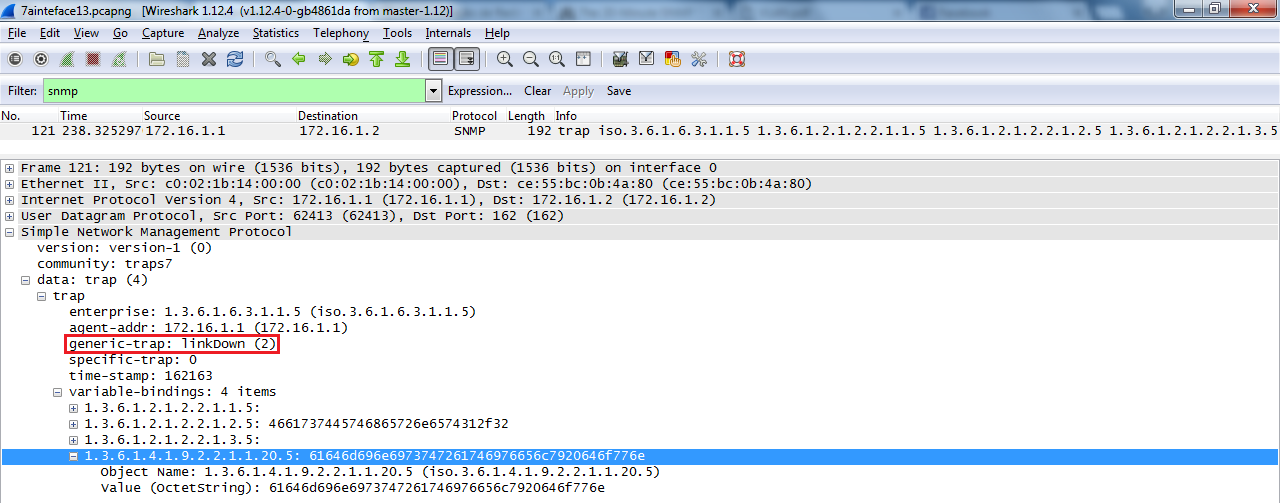
\includegraphics[width=1\textwidth, height=0.33\textheight]{7a.png}
\label{fig:10-capturaWireshark}
\caption{Captura \emph{wireshark} na interface \textsf{1/3} de \textsf{R1}.}
\end{figure}


\subparagraph{b.}
Captura de pacotes SNMP na interface \textsf{f1/3} de \textsf{R1}:

\begin{figure}[h]
\centering
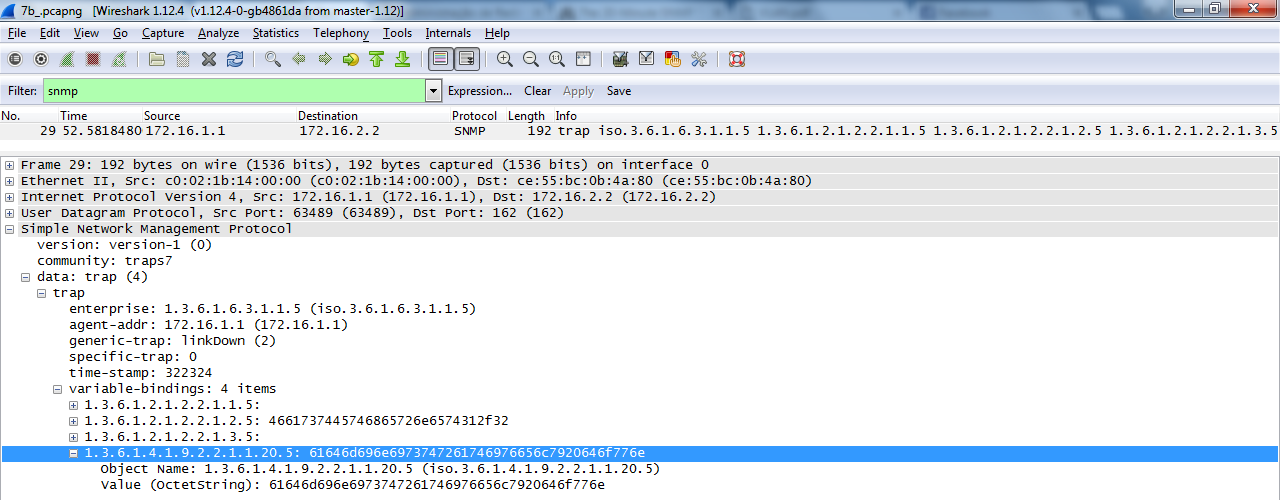
\includegraphics[width=1\textwidth, height=0.33\textheight]{7b.png}
\label{fig:11-capturaWireshark}
\caption{Captura \emph{wireshark} na interface \textsf{1/3} de \textsf{R1}.}
\end{figure}


\subparagraph{c.}
Captura de pacotes SNMP na interface \textsf{f1/3} de \textsf{R1}:

\begin{figure}[h]
\centering
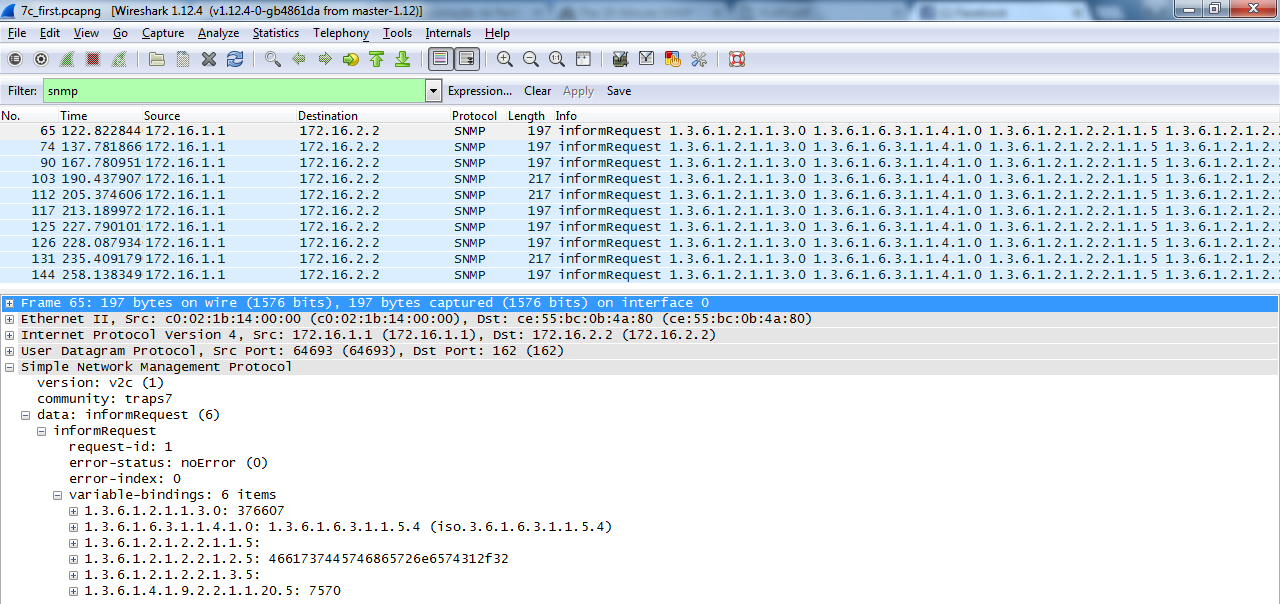
\includegraphics[width=1\textwidth, height=0.33\textheight]{7c.png}
\label{fig:12-capturaWireshark}
\caption{Captura \emph{wireshark} na interface \textsf{1/3} de \textsf{R1}.}
\end{figure}


\subparagraph{d.}
Captura de pacotes SNMP na interface \textsf{f1/3} de \textsf{R1}:

\begin{figure}[h]
\centering
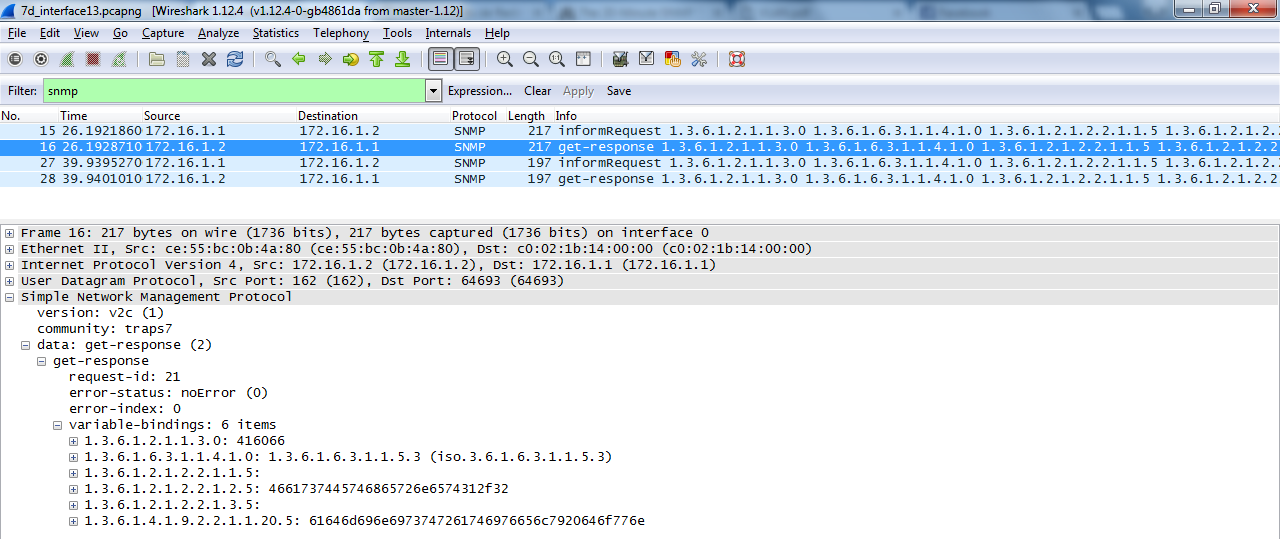
\includegraphics[width=1\textwidth, height=0.33\textheight]{7d.png}
\label{fig:13-capturaWireshark}
\caption{Captura \emph{wireshark} na interface \textsf{1/3} de \textsf{R1}.}
\end{figure}


\subparagraph{e.}
Com base nas alíneas anteriores, comente as diferenças entre o uso de informs e de traps, bem como as implicações práticas dessas diferenças. (texRes)


\paragraph{8.}

\subparagraph{a.}
Captura dos pacotes trocados quando executados os seguintes comandos:

\begin{itemize}
\item \texttt{snmpgetnext -v2c -c Leitura 172.16.1.1 system.sysName}:

\begin{figure}[h]
\centering
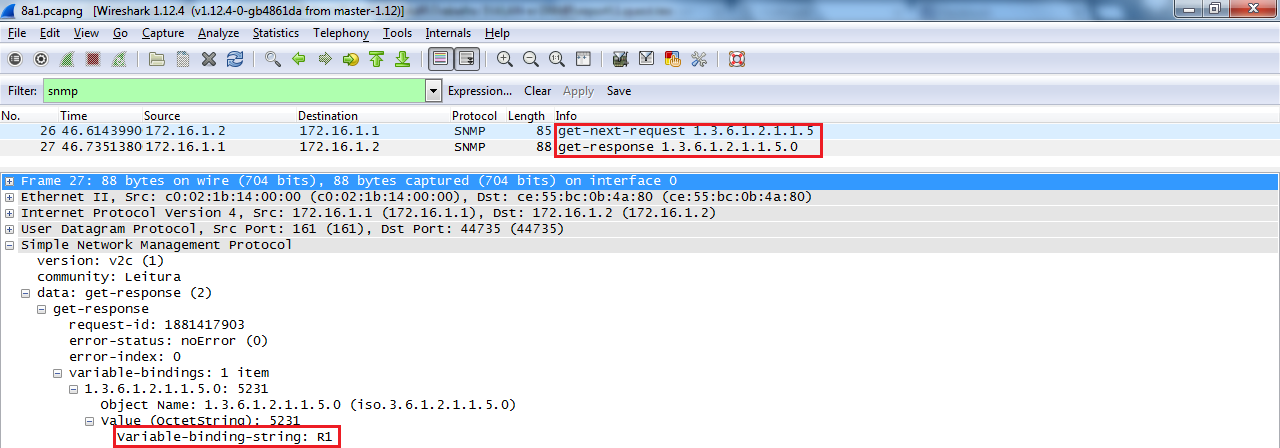
\includegraphics[width=1\textwidth, height=0.33\textheight]{8a1.png}
\label{fig:14-capturaWireshark}
\caption{Captura \emph{wireshark} na interface \textsf{1/3} de \textsf{R1}.}
\end{figure}


\item \texttt{snmpgetnext -v3 -l authNoPriv -u grupo11 -a md5 -A passlimi 172.16.1.1 system.sysName}:

\begin{figure}[h]
\centering
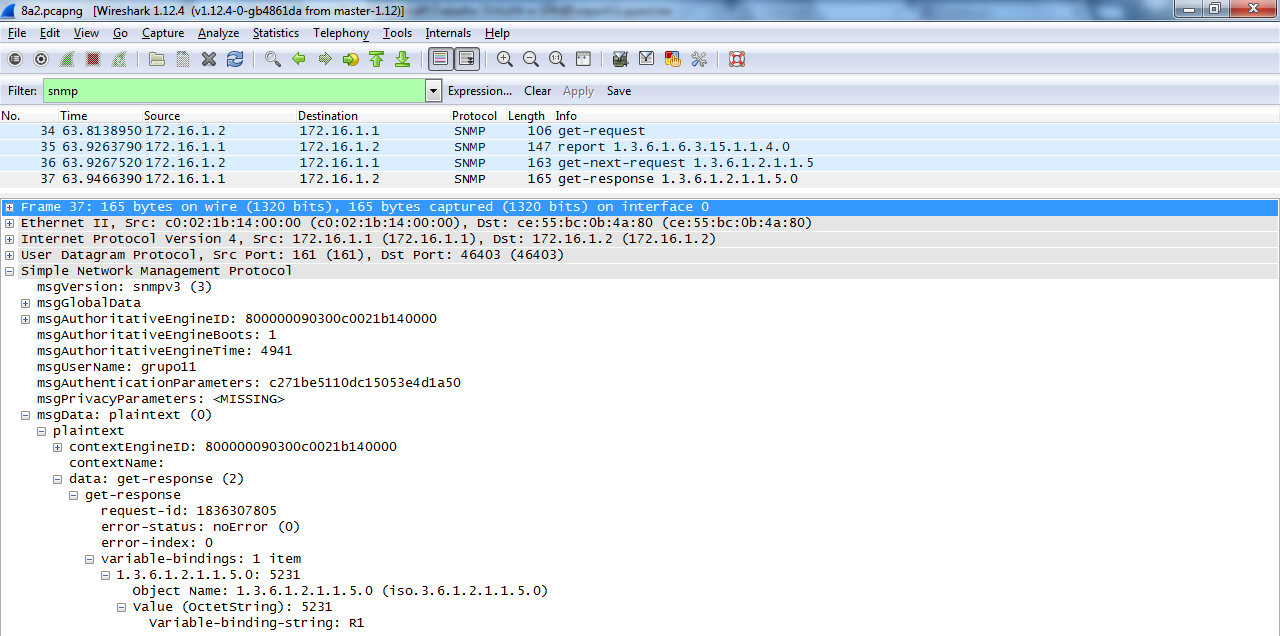
\includegraphics[width=1\textwidth, height=0.33\textheight]{8a2.png}
\label{fig:15-capturaWireshark}
\caption{Captura \emph{wireshark} na interface \textsf{1/3} de \textsf{R1}.}
\end{figure}


\item \texttt{snmpgetnext -v3 -l authPriv -u cifragrupo11 -a md5 -A passlimi -x des -X cifralimi 172.16.1.1 system.sysName}:

\begin{figure}[h]
\centering
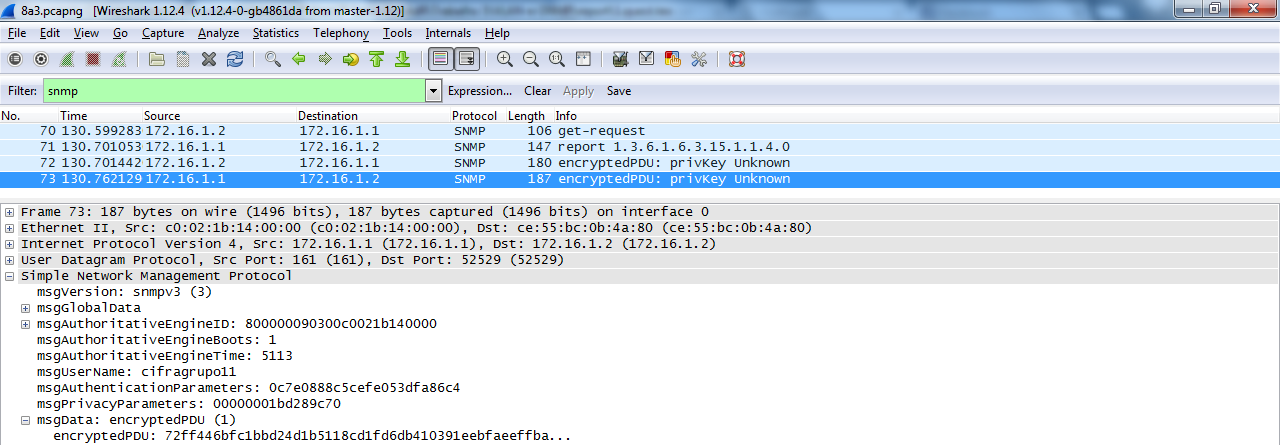
\includegraphics[width=1\textwidth, height=0.33\textheight]{8a3.png}
\label{fig:16-capturaWireshark}
\caption{Captura \emph{wireshark} na interface \textsf{1/3} de \textsf{R1}.}
\end{figure}

\end{itemize}


\subparagraph{b.}
Compare a segurança nos três casos. (texRes)
%\listoffigures
%\listoftables
%\listofalgorithms
\bibliographystyle{acm}
\bibliography{bibl.tex}
\end{document}
